%%%%%%%%%%%%%%%%%%%%%%%%%%%%%%%%%%%%%%%%%
% Programming/Coding Assignment
% LaTeX Template
%
% This template has been downloaded from:
% http://www.latextemplates.com
%
% Original author:
% Ted Pavlic (http://www.tedpavlic.com)
%
% Note:
% The \lipsum[#] commands throughout this template generate dummy text
% to fill the template out. These commands should all be removed when 
% writing assignment content.
%
% This template uses a Perl script as an example snippet of code, most other
% languages are also usable. Configure them in the "CODE INCLUSION 
% CONFIGURATION" section.
%
%%%%%%%%%%%%%%%%%%%%%%%%%%%%%%%%%%%%%%%%%

%----------------------------------------------------------------------------------------
%	PACKAGES AND OTHER DOCUMENT CONFIGURATIONS
%----------------------------------------------------------------------------------------

\documentclass{article}

\usepackage{fancyhdr} % Required for custom headers
\usepackage{lastpage} % Required to determine the last page for the footer
\usepackage{extramarks} % Required for headers and footers
\usepackage[usenames,dvipsnames]{color} % Required for custom colors
\usepackage{graphicx} % Required to insert images
\usepackage{listings} % Required for insertion of code
\usepackage{courier} % Required for the courier font
\usepackage{lipsum} % Used for inserting dummy 'Lorem ipsum' text into the template
\usepackage{multicol} 

\usepackage{tikz}
\usetikzlibrary{arrows,calc} 

\usepackage{quoting}
\quotingsetup{vskip=0pt}

\usepackage[plain]{algorithm}
\usepackage{algpseudocode}
\usepackage{subcaption}

\usepackage{mathtools}
\usepackage{amsmath, amsthm, amssymb}
\usepackage[ansinew]{inputenc}

\makeatletter
\renewcommand{\boxed}[1]{\text{\fboxsep=.2em\fbox{\m@th$\displaystyle#1$}}}
\makeatother

% Margins
\topmargin=-0.45in
\evensidemargin=0in
\oddsidemargin=0in
\textwidth=6.5in
\textheight=9.0in
\headsep=0.25in

\linespread{1.1} % Line spacing

% Set up the header and footer
\pagestyle{fancy}
\lhead{\hmwkAuthorName} % Top left header
\chead{\hmwkClass: \hmwkTitle} % Top center head
\rhead{}
\cfoot{} % Bottom center footer
\rfoot{Page\ \thepage\ of\ \protect\pageref{LastPage}} % Bottom right footer
\renewcommand\headrulewidth{0.4pt} % Size of the header rule
\renewcommand\footrulewidth{0.4pt} % Size of the footer rule

\setlength\parindent{0pt} % Removes all indentation from paragraphs

%----------------------------------------------------------------------------------------
%	CODE INCLUSION CONFIGURATION
%----------------------------------------------------------------------------------------

\definecolor{MyDarkGreen}{rgb}{0.0,0.4,0.0} % This is the color used for comments
\lstloadlanguages{Perl} % Load Perl syntax for listings, for a list of other languages supported see: ftp://ftp.tex.ac.uk/tex-archive/macros/latex/contrib/listings/listings.pdf
\lstset{language=Perl, % Use Perl in this example
        frame=single, % Single frame around code
        basicstyle=\small\ttfamily, % Use small true type font
        keywordstyle=[1]\color{Blue}\bf, % Perl functions bold and blue
        keywordstyle=[2]\color{Purple}, % Perl function arguments purple
        keywordstyle=[3]\color{Blue}\underbar, % Custom functions underlined and blue
        identifierstyle=, % Nothing special about identifiers                                         
        commentstyle=\usefont{T1}{pcr}{m}{sl}\color{MyDarkGreen}\small, % Comments small dark green courier font
        stringstyle=\color{Purple}, % Strings are purple
        showstringspaces=false, % Don't put marks in string spaces
        tabsize=5, % 5 spaces per tab
        %
        % Put standard Perl functions not included in the default language here
        morekeywords={rand},
        %
        % Put Perl function parameters here
        morekeywords=[2]{on, off, interp},
        %
        % Put user defined functions here
        morekeywords=[3]{test},
       	%
        morecomment=[l][\color{Blue}]{...}, % Line continuation (...) like blue comment
        numbers=left, % Line numbers on left
        firstnumber=1, % Line numbers start with line 1
        numberstyle=\tiny\color{Blue}, % Line numbers are blue and small
        stepnumber=5 % Line numbers go in steps of 5
}

% Creates a new command to include a perl script, the first parameter is the filename of the script (without .pl), the second parameter is the caption
\newcommand{\perlscript}[2]{
\begin{itemize}
\item[]\lstinputlisting[caption=#2,label=#1]{#1.pl}
\end{itemize}
}

%----------------------------------------------------------------------------------------
%	DOCUMENT STRUCTURE COMMANDS
%	Skip this unless you know what you're doing
%----------------------------------------------------------------------------------------

% Header and footer for when a page split occurs within a problem environment
\newcommand{\enterProblemHeader}[1]{
\nobreak\extramarks{#1}{#1 continued on next page\ldots}\nobreak
\nobreak\extramarks{#1 (continued)}{#1 continued on next page\ldots}\nobreak
}

% Header and footer for when a page split occurs between problem environments
\newcommand{\exitProblemHeader}[1]{
\nobreak\extramarks{#1 (continued)}{#1 continued on next page\ldots}\nobreak
\nobreak\extramarks{#1}{}\nobreak
}

\setcounter{secnumdepth}{0} % Removes default section numbers
\newcounter{homeworkProblemCounter} % Creates a counter to keep track of the number of problems

\newcommand{\homeworkProblemName}{}
\newenvironment{homeworkProblem}[1][Question \arabic{homeworkProblemCounter}]{ % Makes a new environment called homeworkProblem which takes 1 argument (custom name) but the default is "Problem #"
\stepcounter{homeworkProblemCounter} % Increase counter for number of problems
\renewcommand{\homeworkProblemName}{#1} % Assign \homeworkProblemName the name of the problem
\section{\homeworkProblemName} % Make a section in the document with the custom problem count
\enterProblemHeader{\homeworkProblemName} % Header and footer within the environment
}{
\exitProblemHeader{\homeworkProblemName} % Header and footer after the environment
}

\newcommand{\problemAnswer}[1]{ % Defines the problem answer command with the content as the only argument
\noindent\framebox[\columnwidth][c]{\begin{minipage}{0.98\columnwidth}#1\end{minipage}} % Makes the box around the problem answer and puts the content inside
}

\newcommand{\homeworkSectionName}{}
\newenvironment{homeworkSection}[1]{ % New environment for sections within homework problems, takes 1 argument - the name of the section
\renewcommand{\homeworkSectionName}{#1} % Assign \homeworkSectionName to the name of the section from the environment argument
\subsection{\homeworkSectionName} % Make a subsection with the custom name of the subsection
\enterProblemHeader{\homeworkProblemName\ [\homeworkSectionName]} % Header and footer within the environment
}{
\enterProblemHeader{\homeworkProblemName} % Header and footer after the environment
}

%----------------------------------------------------------------------------------------
%	NAME AND CLASS SECTION
%----------------------------------------------------------------------------------------

\newcommand{\hmwkTitle}{Assignment\ \#1} % Assignment title
\newcommand{\hmwkDueDate}{Monday, 16\textsuperscript{th} of May, 2016} % Due date
\newcommand{\hmwkClass}{Design and Analysis of Algorithms} % Course/class
\newcommand{\hmwkClassTime}{4:00pm} % Class/lecture time
\newcommand{\hmwkClassInstructor}{Jones} % Teacher/lecturer
\newcommand{\hmwkAuthorName}{Tim Cochrane} % Your name
\newcommand{\studentNum}{17766247}

%----------------------------------------------------------------------------------------
%	TITLE PAGE
%----------------------------------------------------------------------------------------

\title{
\vspace{2in}
\textmd{\textbf{\hmwkClass}}\\
\textmd{\hmwkTitle}\\
\normalsize\vspace{0.1in}\small{\hmwkDueDate}\\
\vspace{3in}
}

\author{\textbf{\hmwkAuthorName} \\ \studentNum}
\date{} % Insert date here if you want it to appear below your name

%----------------------------------------------------------------------------------------

\begin{document} 
\maketitle\thispagestyle{empty}

%----------------------------------------------------------------------------------------
%	TABLE OF CONTENTS
%----------------------------------------------------------------------------------------

%\setcounter{tocdepth}{1} % Uncomment this line if you don't want subsections listed in the ToC

%  \newpage
%  \tableofcontents
%  \newpage

\clearpage
\setcounter{page}{1}

%----------------------------------------------------------------------------------------
%	PROBLEM 1
%----------------------------------------------------------------------------------------

% To have just one problem per page, simply put a \clearpage after each problem

\begin{homeworkProblem}

    a) Use the Master method solve the folloing recurrence function:
    \begin{center}
        $T(n) = 3T(\sqrt[2]{n}) + \log_2{n}$
    \end{center}
    \textbf{Solution}
    \begin{quoting}
        \abovedisplayskip=0pt
        \begin{align}
            \shortintertext{Inital recurance:}
            T(n) & = 3T(\sqrt[2]{n}) + \log_2{n} \notag \\
            \shortintertext{Substitute for $k = \log_2{n}$:}
            T(2^k) & = 3T(2^{\frac{k}{2}}) + k \notag \\
            \shortintertext{Now in the master thereom form:}
            T(n) & = aT(n/b) + f(n) \notag \\
            \shortintertext{Where:}
            a = 3, b & = 2, f(n) = k \notag
            \shortintertext{Checking which master thereom case to use:}
            k^{\log_b{a}} & = k^{\log_2{3}} \approx k^{1.6} \notag \\
            k^{1} & < k^{1.6} \notag
        \end{align}
        \begin{center}
            $\therefore$ case 1 of master thereom \\
            The solution to the recurance is $O(n^{\log_2{3}})$.
        \end{center}
    \end{quoting}
    \vskip0.5cm
   %\begin{align}
   %    \sqrt{k} = \sqrt{\log_2{n}} = 2^{\frac{\log_2{n}}{2}} = 2^\frac{k}{2}
   %\end{align}

    b) Consider the recurrence function $T(n) = 2T(n-1)+1$ state the upper 
    bound time complexity of the function and use induction to 
    prove that the time complexity is correct. \\

    \textbf{Solution}

    \begin{quoting}
        Assuming that $T(1) = 1$ lets calculate the first few values of the
        the recurrance to get an idea of the function.
        \begin{align}
            T(1) & = 1 \notag \\
            T(2) & = 2(1) + 1 = 3 \notag \\
            T(3) & = 2(3) + 1 = 7 \notag \\
            T(4) & = 2(7) + 1 = 15 \notag
        \end{align}

        The initial values of the recurrance appears to be $2^{n} - 1$. Lets
        try and prove this by induction. \\

        \textbf{Inductive Hypothesis}
        \begin{center}
            $T(n) \in O(2^{n} - 1)$
        \end{center}
        \textbf{Base Case}
        \begin{align}
            T(2) & = 2T(2 - 1) + 1 & 2^{2} - 1 & = 4 - 1 \notag \\
                 & = 2T(1) + 1 & & = 3 \notag \\
                 & = 2 + 1 = 3 & & = 3 \notag
        \end{align}
        \begin{center}
            $\therefore$ \text{base case holds}
        \end{center}

        \textbf{Inductive Step}
        \begin{align}
            T(n + 1) & = 2T(n + 1 - 1) + 1 \notag \\
                     & = 2T(n) + 1 \notag \\
                     & = 2(2^{n} - 1) + 1 \notag \\
                     & = 2^{n+1} - 2 + 1 \notag \\
                     & = 2^{n+1} - 1 \notag 
        \end{align}
        \begin{center}
            Same form as our hypothesis
        \end{center}
        \vskip0.5cm
        We have proven through induction that the recurance has an upper 
        bound time complexity of $O(2^n)$.
    \end{quoting}

\end{homeworkProblem}

%----------------------------------------------------------------------------------------
%	PROBLEM 2
%----------------------------------------------------------------------------------------

\begin{homeworkProblem}
    \begin{figure}[H]
        \begin{center}
            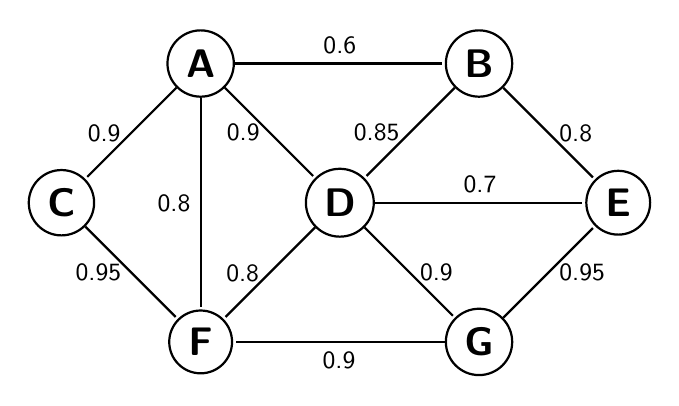
\begin{tikzpicture}[>=stealth',shorten >=1pt,auto,node distance=2.5cm,
                thick,main node/.style={circle,draw,font=\sffamily\Large\bfseries}]

                \node[main node] (A) {A};
                \node[main node] (D) [below right of=A]{D};
                \node[main node] (B) [above right of=D]{B};
                \node[main node] (C) [below left of=A]{C};
                \node[main node] (E) [below right of=B]{E};
                \node[main node] (F) [below left of=D]{F};
                \node[main node] (G) [below right of=D]{G};

                \path[every node/.style={font=\sffamily\small}]
                (A) edge node [left] {0.9} (C)
                    edge node [left] {0.8} (F)
                    edge node [left] {0.9} (D)
                    edge node [above] {0.6} (B)
                (B) edge node [left] {0.85} (D)
                    edge node [right] {0.8} (E)
                (C) edge node [left] {0.95} (F)
                (D) edge node [above] {0.7} (E)
                    edge node [right] {0.9} (G)
                    edge node [left] {0.8} (F)
                (G) edge node [below] {0.9} (F)
                    edge node [right] {0.95} (E);
            \end{tikzpicture}
        \end{center}
        \caption{Undirected weighted graph}
        \belowcaptionskip0cm
        \label{graph1}
    \end{figure}

    a) Design a \textit{greedy} algorithm that generates the most reliable path from
    a source node s to every destination node $t$ in the network. Show your algorithm
    in a concise and clear pseudo-code. Further, you must explain in detail each line
    of your pseudo-code and show how to implement your algorithm so that it has the
    best possible time complexity. \\

    \textbf{Solution}
    \begin{algorithm}[H]
        \begin{algorithmic}[1]
            \Function{Dijkstra}{$G, w, s$}
            \State{} \Call{Initialize-Single-Source}{$G, s$}
            \State{} $S = \emptyset$
            \State{} $Q = G.V$
                \While{$Q \neq \emptyset$}
                    \State{} $u = \Call{Extract-Max}{$Q$} $
                    \State{} $S = S \cup \{u\}$
                    \For{each vertex $v \in G.Adj[u]$}
                        \State{} \Call{Tense}{$u,v,w$}
                    \EndFor
                \EndWhile \EndFunction{}
        \end{algorithmic}
        \caption{Modified Dijkstra's Algorithm}
        \label{alg:path}
    \end{algorithm}
    \begin{algorithm}[H]
        \begin{algorithmic}[1]
            \Function{Initialize-Single-Source}{$G, s$}
                \For{each vertex $v \in G.V$}
                    \State{} $v.d = \infty$
                    \State{} $v.\pi = NIL$
                \EndFor
            \State{} $s.d = 1$
            \EndFunction
        \end{algorithmic}
        \caption{Initialize our vertex's}
    \end{algorithm}
    \begin{algorithm}[H]
        \begin{algorithmic}[1]
            \Function{Tense}{$u, v, w$}
                \If{$v.d < u.d * w(u,v)$}
                    \State{} $v.d = u.d * w(u,v)$
                    \State{} $v.\pi = u$
                \EndIf
            \EndFunction{}
        \end{algorithmic}
        \caption{Modified Relax Algorithm}
    \end{algorithm}

    \vskip0.5cm

    b) Use your algorithm in part a) to generate the most reliable path from
    node A to every other node for the given graph. List the most reliable paths and
    their corresponding path reliabilities. 

    \begin{figure}[H]
        \begin{center}
            \begin{tabular}{*{8}{c |}}
                & $A$ & $B$ & $C$ & $D$ & $E$ & $F$ & $G$ \\
            \hline
        $A$ & $\boxed{1}$ & $0.6$ & $0.9$ & $0.9$ & $\infty$ & $0.8$ & $\infty$ \\
        $C$ & $1$ & $0.6$ & $\boxed{0.9}$ & $0.9$ & $\infty$ & $0.855$ & $\infty$ \\
        $D$ & $1$ & $0.765$ & $0.9$ & $\boxed{0.9}$ & $0.63$ & $0.855$ & $0.81$ \\
        $F$ & $1$ & $0.765$ & $0.9$ & $0.9$ & $0.63$ & $\boxed{0.855}$ & $0.81$ \\
        $G$ & $1$ & $0.765$ & $0.9$ & $0.9$ & $0.7695$ & $0.8$ & $\boxed{0.81}$ \\
        $E$ & $1$ & $0.765$ & $0.9$ & $0.9$ & $\boxed{0.7695}$ & $0.8$ & $0.81$ \\
        $B$ & $1$ & $\boxed{0.765}$ & $0.9$ & $0.9$ & $0.7695$ & $0.8$ & $0.81$ \\
            \end{tabular}
            \caption{Result of Algorithm~\ref{alg:path}}
            \label{path_result}
        \end{center}
    \end{figure}

    \begin{quoting}
        From the algorithm we have found the following paths to each node:
        \begin{align}
            B:&  \{A \to D \to B\} = 0.765 \notag \\
            C:&  \{A \to C\} = 0.9  \notag \\
            D:&  \{A \to D\} = 0.9  \notag \\
            E:&  \{A \to D \to G \to E\} = 0.7695 \notag \\
            F:&  \{A \to C \to F \} = 0.855 \notag \\
            G:&  \{A \to D \to G \} = 0.81 \notag
        \end{align}
    \end{quoting}
\end{homeworkProblem}

%----------------------------------------------------------------------------------------

\begin{homeworkProblem}
    \begin{figure}[H]
        \begin{center}
            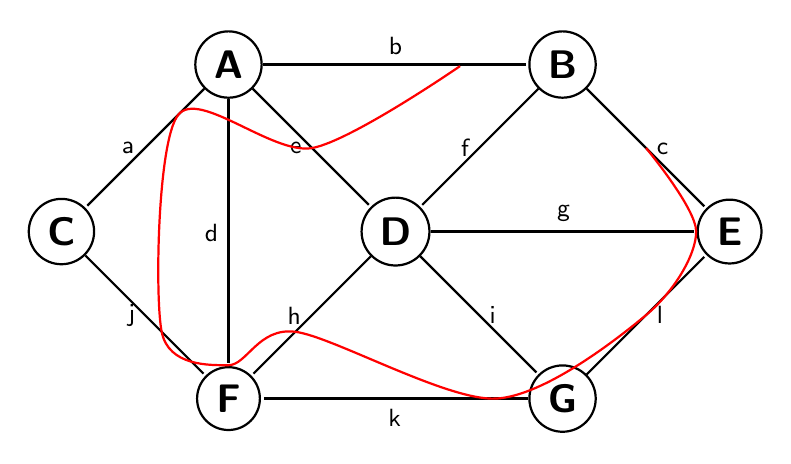
\begin{tikzpicture}[>=stealth',shorten >=1pt,auto,node distance=3cm,
                thick,main node/.style={circle,draw,font=\sffamily\Large\bfseries}]

                \node[main node] (A) {A};
                \node[main node] (D) [below right of=A]{D};
                \node[main node] (B) [above right of=D]{B};
                \node[main node] (C) [below left of=A]{C};
                \node[main node] (E) [below right of=B]{E};
                \node[main node] (F) [below left of=D]{F};
                \node[main node] (G) [below right of=D]{G};

                \path[every node/.style={font=\sffamily\small}]
                (A) edge node [left] {a} (C)
                    edge node [left] {d} (F)
                    edge node [left] {e} (D)
                    edge node [above] {b} (B)
                (B) edge node [left] {f} (D)
                    edge node [right] {c} (E)
                (C) edge node [left] {j} (F)
                (D) edge node [above] {g} (E)
                    edge node [right] {i} (G)
                    edge node [left] {h} (F)
                (G) edge node [below] {k} (F)
                    edge node [right] {l} (E);

                    \draw [red] plot [smooth,tension=0.5] coordinates {
                    ($ (B) !.5! (E) $) 
                    ($ (D) !.9! (E) $) 
                    ($ (E) !.5! (G) $) 
                    ($ (F) !.8! (G) $)
                    ($ (D) !.6! (F) $)
                    ($ (A) !.9! (F) $)
                    ($ (C) !.6! (F) $)
                    ($ (C) !.7! (A) $)
                    ($ (A) !.5! (D) $)
                    ($ (A) !.7! (B) $)};
            \end{tikzpicture}
        \end{center}
        \caption{Undirected weighted graph}
        \belowcaptionskip0cm
        \label{graph2}
    \end{figure}

    a) Generate all possible cuts in the given graph, and determine its
    maximum cut. \\

    \begin{quoting}
        After generating all of the possible cuts, I found the largest cut
        had a size of 9 and occured with the following subsets.

        \begin{center}
            $s_1 = \{B,C,D,G\}, s_2 = \{A,E,F\}$
        \end{center}

        The order of these subsets is irrelivent as flipping the variables
        will still produce the same cut.

        \pagebreak
        \textbf{All possible cuts of a 7 vertex graph.} \\
        The number of subgraphs possible for any given graph
        is defined as $2^{n} - 2$ but we only need half of 
        theses as changing the order of the variables does 
        not produce any new cuts.
        \begin{multicols}{2}
            \begin{tabular}{l l | }
                $\{B,C,D,E,F,G\}$ &$\{A\}$ \\
                $\{A,C,D,E,F,G\}$ &$\{B\}$ \\
                $\{C,D,E,F,G\}$ &$\{A,B\}$ \\
                $\{A,B,D,E,F,G\}$ &$\{C\}$ \\
                $\{B,D,E,F,G\}$ &$\{A,C\}$ \\
                $\{A,D,E,F,G\}$ &$\{B,C\}$ \\
                $\{D,E,F,G\}$ &$\{A,B,C\}$ \\
                $\{A,B,C,E,F,G\}$ &$\{D\}$ \\
                $\{B,C,E,F,G\}$ &$\{A,D\}$ \\
                $\{A,C,E,F,G\}$ &$\{B,D\}$ \\
                $\{C,E,F,G\}$ &$\{A,B,D\}$ \\
                $\{A,B,E,F,G\}$ &$\{C,D\}$ \\
                $\{B,E,F,G\}$ &$\{A,C,D\}$ \\
                $\{A,E,F,G\}$ &$\{B,C,D\}$ \\
                $\{E,F,G\}$ &$\{A,B,C,D\}$ \\
                $\{A,B,C,D,F,G\}$ &$\{E\}$ \\
                $\{B,C,D,F,G\}$ &$\{A,E\}$ \\
                $\{A,C,D,F,G\}$ &$\{B,E\}$ \\
                $\{C,D,F,G\}$ &$\{A,B,E\}$ \\
                $\{A,B,D,F,G\}$ &$\{C,E\}$ \\
                $\{B,D,F,G\}$ &$\{A,C,E\}$ \\
                $\{A,D,F,G\}$ &$\{B,C,E\}$ \\
                $\{D,F,G\}$ &$\{A,B,C,E\}$ \\
                $\{A,B,C,F,G\}$ &$\{D,E\}$ \\
                $\{B,C,F,G\}$ &$\{A,D,E\}$ \\
                $\{A,C,F,G\}$ &$\{B,D,E\}$ \\
                $\{C,F,G\}$ &$\{A,B,D,E\}$ \\
                $\{A,B,F,G\}$ &$\{C,D,E\}$ \\
                $\{B,F,G\}$ &$\{A,C,D,E\}$ \\
                $\{A,F,G\}$ &$\{B,C,D,E\}$ \\
                $\{F,G\}$ &$\{A,B,C,D,E\}$ \\
            \end{tabular}
            \begin{tabular}{l l}
                $\{A,B,C,D,E,G\}$ &$\{F\}$ \\
                $\{B,C,D,E,G\}$ &$\{A,F\}$ \\
                $\{A,C,D,E,G\}$ &$\{B,F\}$ \\
                $\{C,D,E,G\}$ &$\{A,B,F\}$ \\
                $\{A,B,D,E,G\}$ &$\{C,F\}$ \\
                $\{B,D,E,G\}$ &$\{A,C,F\}$ \\
                $\{A,D,E,G\}$ &$\{B,C,F\}$ \\
                $\{D,E,G\}$ &$\{A,B,C,F\}$ \\
                $\{A,B,C,E,G\}$ &$\{D,F\}$ \\
                $\{B,C,E,G\}$ &$\{A,D,F\}$ \\
                $\{A,C,E,G\}$ &$\{B,D,F\}$ \\
                $\{C,E,G\}$ &$\{A,B,D,F\}$ \\
                $\{A,B,E,G\}$ &$\{C,D,F\}$ \\
                $\{B,E,G\}$ &$\{A,C,D,F\}$ \\
                $\{A,E,G\}$ &$\{B,C,D,F\}$ \\
                $\{E,G\}$ &$\{A,B,C,D,F\}$ \\
                $\{A,B,C,D,G\}$ &$\{E,F\}$ \\
                $\{B,C,D,G\}$ &$\{A,E,F\}$ \\
                $\{A,C,D,G\}$ &$\{B,E,F\}$ \\
                $\{C,D,G\}$ &$\{A,B,E,F\}$ \\
                $\{A,B,D,G\}$ &$\{C,E,F\}$ \\
                $\{B,D,G\}$ &$\{A,C,E,F\}$ \\
                $\{A,D,G\}$ &$\{B,C,E,F\}$ \\
                $\{D,G\}$ &$\{A,B,C,E,F\}$ \\
                $\{A,B,C,G\}$ &$\{D,E,F\}$ \\
                $\{B,C,G\}$ &$\{A,D,E,F\}$ \\
                $\{A,C,G\}$ &$\{B,D,E,F\}$ \\
                $\{C,G\}$ &$\{A,B,D,E,F\}$ \\
                $\{A,B,G\}$ &$\{C,D,E,F\}$ \\
                $\{B,G\}$ &$\{A,C,D,E,F\}$ \\
                $\{A,G\}$ &$\{B,C,D,E,F\}$ \\
                $\{G\}$ &$\{A,B,C,D,E,F\}$ \\
            \end{tabular}
        \end{multicols}
    \end{quoting}

    b) Design a greedy algorithm to solve the Max-Cut problem. As part of
    your solution, you must state your greedy criteria. Further, show your algorithm
    in a concise but clear pseudo-code. You must explain in detail each line of the
    pseudo-code and show how to implement the algorithm so that it has the best
    possible time complexity. \\

    \begin{quoting}

        My algorithm will attempt to find the soltion to the Max Cut problem
        by greedily selecting the vertex with the next highest degree,
        ignoring previously cut links, and checking if swapping the subset it
        belongs to will increase the max cut.

        \begin{algorithm}[H]
            \begin{algorithmic}[1]
                \Function{MaxCut}{$G, V, E$}
                \State{} $subSet = \emptyset$ \Comment{Declare a variable to store the subset we will be checking.}
                \State{} $innerDegree = \emptyset$ \Comment{A variable to store our calculated inner degree.}

                \State{} \Call{Randomize-Sets}{$V, subSet$} \Comment{Split the vertex's into a random pair of subsets.} \\

                \For{each vertex $V$ as $vertex$} \Comment{For each vertex in the graph}
                    \For{each $vertex.Adj$ as $edge$} \Comment{For each connected node of that vertex.}
                        \If{\Call{In-Set}{$vertex, subSet$} $=$ \Call{In-Set}{$edge, subSet$}} \Comment{If they are in the same subset}
                            \State{} $innerDegre.vertex = innerDegree.vertex + 1$ \Comment{Increment innerDegree}
                        \EndIf{}
                    \EndFor{}
                \EndFor{} \\

                \For{each $vertex$ within $innerDegree$ in descending order}
                \State{} $oldSubSet = subSet$ \Comment{Keep track of last known cut}
                    \State{} $curCut = \Call{calculateCut}{}$

                    \If{$\Call{inSet}{vertex, subSet}$}
                        \State{} $S = S - \{vertex\}$ \Comment{Remove the current vertex from the subset}
                    \Else{}
                        \State{} $S = S \cup \{vertex\}$ \Comment{Add the current vertex to the subset}
                    \EndIf{}

                    \If{$\Call{calculateCut}{} < curCut$} \Comment{We have increased the cut by switching}
                    curCut = \Call{calculateCut}{} \Comment{Update the highest found cut
                    \Else{}
                    \Endif{}
                \EndFor{}

                \State{} 
                \EndFunction{}
            \end{algorithmic}
            \caption{Greedy algorithm to solve the MaxCut Problem}
        \end{algorithm}
        
    \end{quoting}

\end{homeworkProblem}

\end{document}
